\section{Introduction}

While techniques for analysing the dependency structure of programs have been fruitful, with applications ranging from information-flow security~\cite{sabelfeld03} and optimisation~\cite{kildall73} to debugging and program comprehension~\cite{weiser81,delucia96}, there are few methods suitable for fine-grained analysis of richly structured outputs such as data visualisations and matrices. There are fewer still that are \emph{bidirectional}, i.e.~that can be run either forwards or backwards through the computation, with round-tripping conditions that relate the two directions. For programs which operate on richly structured data, such as visualisation code which turns tables of data into charts, users need to be able to focus on a particular part of the output, and isolate the input data pertinent only to that substructure. Bidirectionality allows these sorts of query to be run in the other direction, but also ensures that the forward and backward analysis are related in a coherent way.

This sort of information is no longer just relevant to programmers. Every day, journalists and scientists curate data into charts and other visual summaries which must be interpreted by colleagues, policy makers and lay readers alike. But charts can be hard to interpret correctly. Innocent (but devastating) mistakes such as transposing two columns of data have gone unnoticed for several years, even in widely cited papers~\cite{miller06}. Less innocent mistakes are deployed by politicians to mislead voters~\cite{fullfact19}. For the sake of transparency and trust, it is imperative that content consumers, as well as content creators, are able to easily verify for themselves what visual summaries actually \emph{represent}. This in turn involves understanding the mapping between data and visual elements, which is a hard task, requiring time and expertise, even with the data and source code used to create the visualisation to hand.

The situation would be much improved if visualisations allowed a reader to explore the relationship to the underlying data through the visualisation itself, revealing the relevant connections on a need-to-know basis, as the reader interacts with it. This is illustrated on the left-hand side of \figref{introduction:vis-linking} below:

\begin{figure}[H]
   {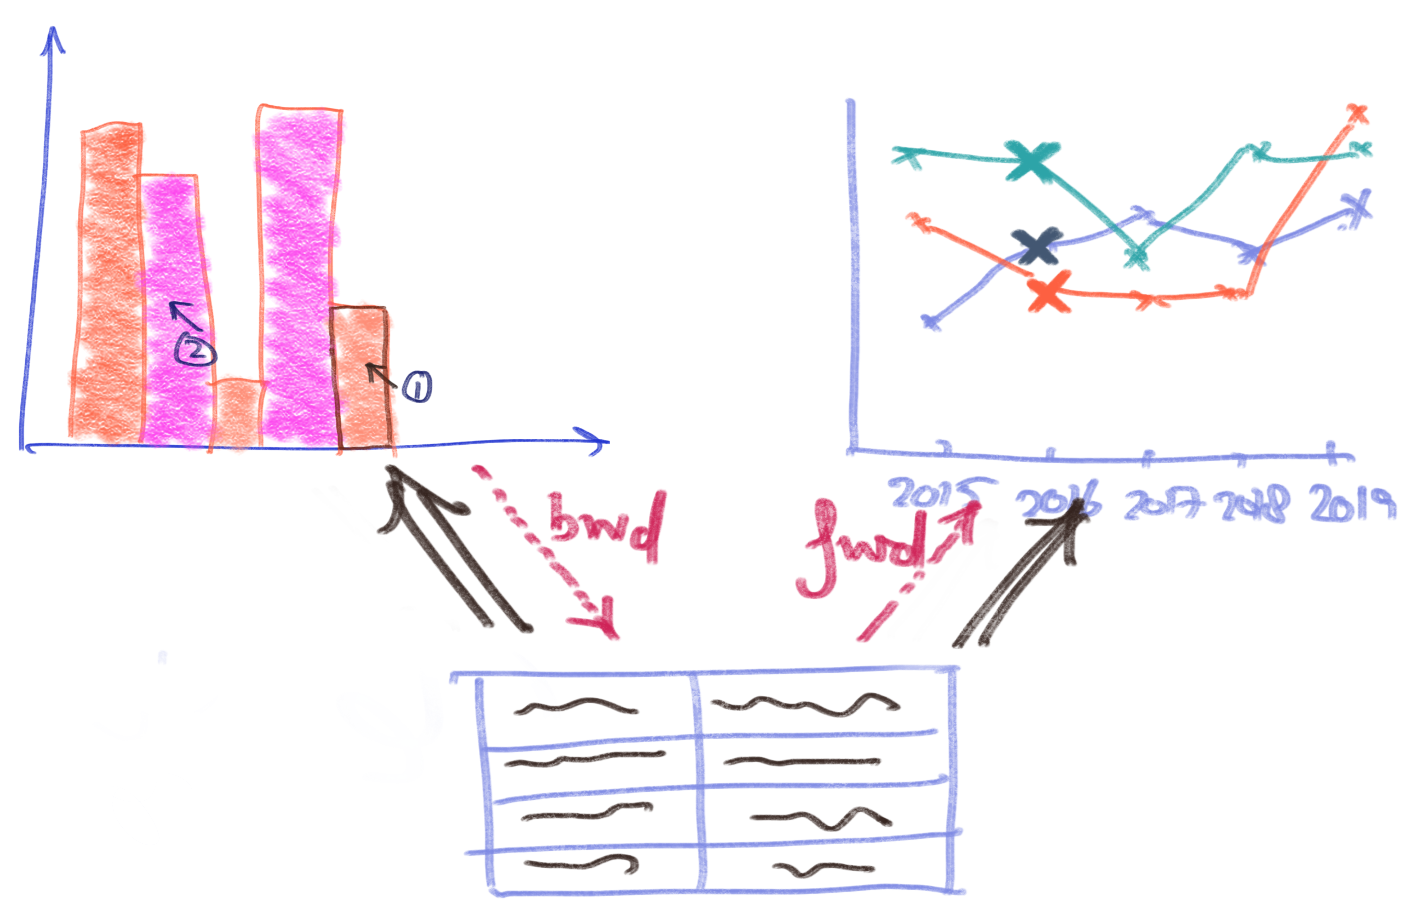
\includegraphics[scale=0.14]{fig/example/vis-linking.png}}
   \small
   \begin{lstlisting}
      let data = [ ... ]
      let barchart = data |> some transformation
      let linechart = data |> some other transformation
   \end{lstlisting}
   \caption{Linking cognate visualisations via common data dependencies}
   \label{fig:introduction:vis-linking}
\end{figure}

\noindent From a program analysis perspective, this presents an interesting problem: we want to be able to focus on a particular visual element, such as a bar in a bar chart, and see what inputs contribute to it. This is a matter of selecting a part of the structured output and performing some kind of backwards analysis that identifies parts of the input data and perhaps parts of the program that contributed to the selected output.

Visualisation designers do sometimes create ``data-linked'' artefacts like these by hand, such as Nadieh Bremer's award-winning visualisation of population density growth in Asian cities~\cite{bremer15}. But crafting such things by hand is a significant undertaking, requiring intimate knowledge of the computational relationship between chart and data, and programming effort to expose that information to the reader. Manual approaches are also error-prone and needs to be changed whenever the application logic changes. A library-based approach would improve on this, but would only provide data linking for solutions that can be readily expressed using the library. By framing this as a program analysis problem, visualisation code can be completely oblivious to these additional transparency features. The data scientist or visualisation designer need concern themselves only with constructing the appropriate view as a function of the data, leaving the programming language to take care of linking the outputs to the data sources in a fine-grained way.

It is also common to use more than one view to present distinct but related aspects of data. (We say visualisations are \emph{cognate} when they are related in this way.) Geospatial applications like GeoDa~\cite{anselin06} and charting libraries like Plotly provide a view coordination feature called \emph{brushing and linking}~\cite{becker87}, where selections in one chart automatically select corresponding elements in the other, as an aid to comprehension. In \figref{introduction:vis-linking} below, selecting a bar on the left automatically selects all the related visual elements on the right. Although such coordination features are highly desirable, they are either baked into specific applications, or require programmer effort and therefore must be anticipated in advance by the chart designer. Moreover the linking is opaque, providing no direct way for the reader to see the data which underpins the relationship.

Problem (2) is more challenging; we want to be able to focus on a visual element in one chart or graphic and see what aspects of a different chart are computed using related inputs. Much work in data visualisation has been done towards this goal, typically done through visualisation libraries rather than program analysis techniques. This is a matter of again selecting a part of the structured output and performing a backwards analysis to identify the required inputs, but then performing a further forwards analysis to identify dependent parts of the other output. The forward analysis part is shown on the right-hand side of \figref{introduction:vis-linking} above.

\hrule

Where-provenance~\cite{buneman01} and related data provenance techniques are fine-grained but are usually restricted to relational query languages. Taint tracking \cite{newsome05} tends to be low-level approach and restricted to tracking taint forwards from input to output. Dataflow analyses \cite{reps95} focus on analysing variables rather than parts of structured values.

Recent program slicing techniques \cite{perera12a,perera13a,ricciotti17} allow the user to focus on the output by ``erasing'' parts deemed to be irrelevant; the erased parts, called \emph{holes}, are propagated backwards by a backwards analysis which identifies parts of the program and input which are no longer needed. Although these approaches enjoy useful round-tripping properties characterised by Galois connections, they only allow focusing on \emph{prefixes} of a structured output, rather than arbitrary substructures.

\subsection{Our contributions}

In this paper, we present new language-based data provenance techniques for linking visualisations to data, and to each other, in a fine-grained way. Our specific contributions are as follows:

\begin{itemize}[leftmargin=*]
   \item[--] a review of \emph{Galois slicing}, a program slicing framework with round-tripping properties appropriate to our problem, and an analysis of its shortcomings (\secref{background});
   \item[--] a new bidirectional dependency analysis inspired by Galois slicing, addressing these shortcomings, for a core calculus with lists and arrays, and a discussion of how the components of this analysis can be combined in various ways to link inputs to outputs and outputs to other outputs (\secref{core-language});
   \item[--] a richer surface language called \OurLanguage with familiar functional programming features, including piecewise definitions, pattern matching, list notation and list comprehensions, and an extension of our analysis to the desugaring (\secref{surface-language});
   \item[--] an implementation of Fluid in PureScript, and a discussion and evaluation of the strengths and weaknesses of our approach (\secref{implementation}).
\end{itemize}
